\section{Evaluation Plan}\label{sec:eval}

\begin{wrapfigure}{r}{3.0in}\centering
\begin{tabular}{cc}
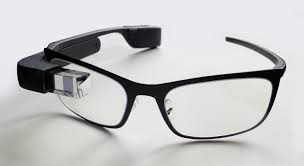
\includegraphics[width=0.45\linewidth]{../figure/glass1.jpg} &
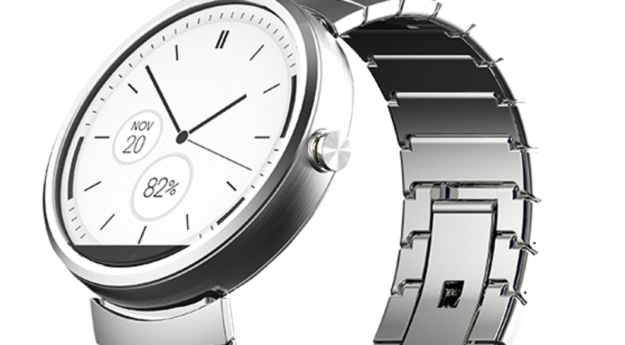
\includegraphics[width=0.45\linewidth]{../figure/moto} \\
(a) & (b) \\
\end{tabular}
    \caption{\label{fig:devices} We will implement~\systemname~on (a) Google Glass and (b) Moto 360 smart watch.}
\vspace{-6pt}
\end{wrapfigure}
\subsection{~\systemname~App on Google Glass and Moto 360}\label{subsec:app}
In this proposal, we propose a body-movement pattern based authentication system, ~\systemname~for 
wearable devices. In addition to developing and evaluating the proposed algorithms, we will also conduct in-depth evaluation of the~\systemname~system design. Even though there are many types of body movements that we can exploit for authentication purposes, in this project we will focus on the movements that can be easily captured by Google Glass (representing smart glasses) and those by Moto 360 (representing smart watches). Specifically, we will study the following movement patterns:
\begin{itemize}
\item \emph{Movement patterns for smart glasses:} As far as smart glasses are concerned, we will explore head movement patterns (with music), eye blinking/winking patterns (with music), and pulses measured at the temple. 

\item \emph{Movement patterns for smart watches:} As far as smart watches are concerned, we will explore arm movement patterns (with music), wrist movement patterns (with music), finger movements (with music), and pulses measured at the wrist.
\end{itemize}  

We will choose easy-to-follow and fast-tempo music tracks (10 seconds long) as external stimuli. The readers can download such an audio track at our web site: \emph{http://www.winlab.rutgers.edu/~sugangli/somebody.midi}. 

\subsection{Data Collection}\label{subsec:user}
\begin{wrapfigure}{r}{3.0in}\centering
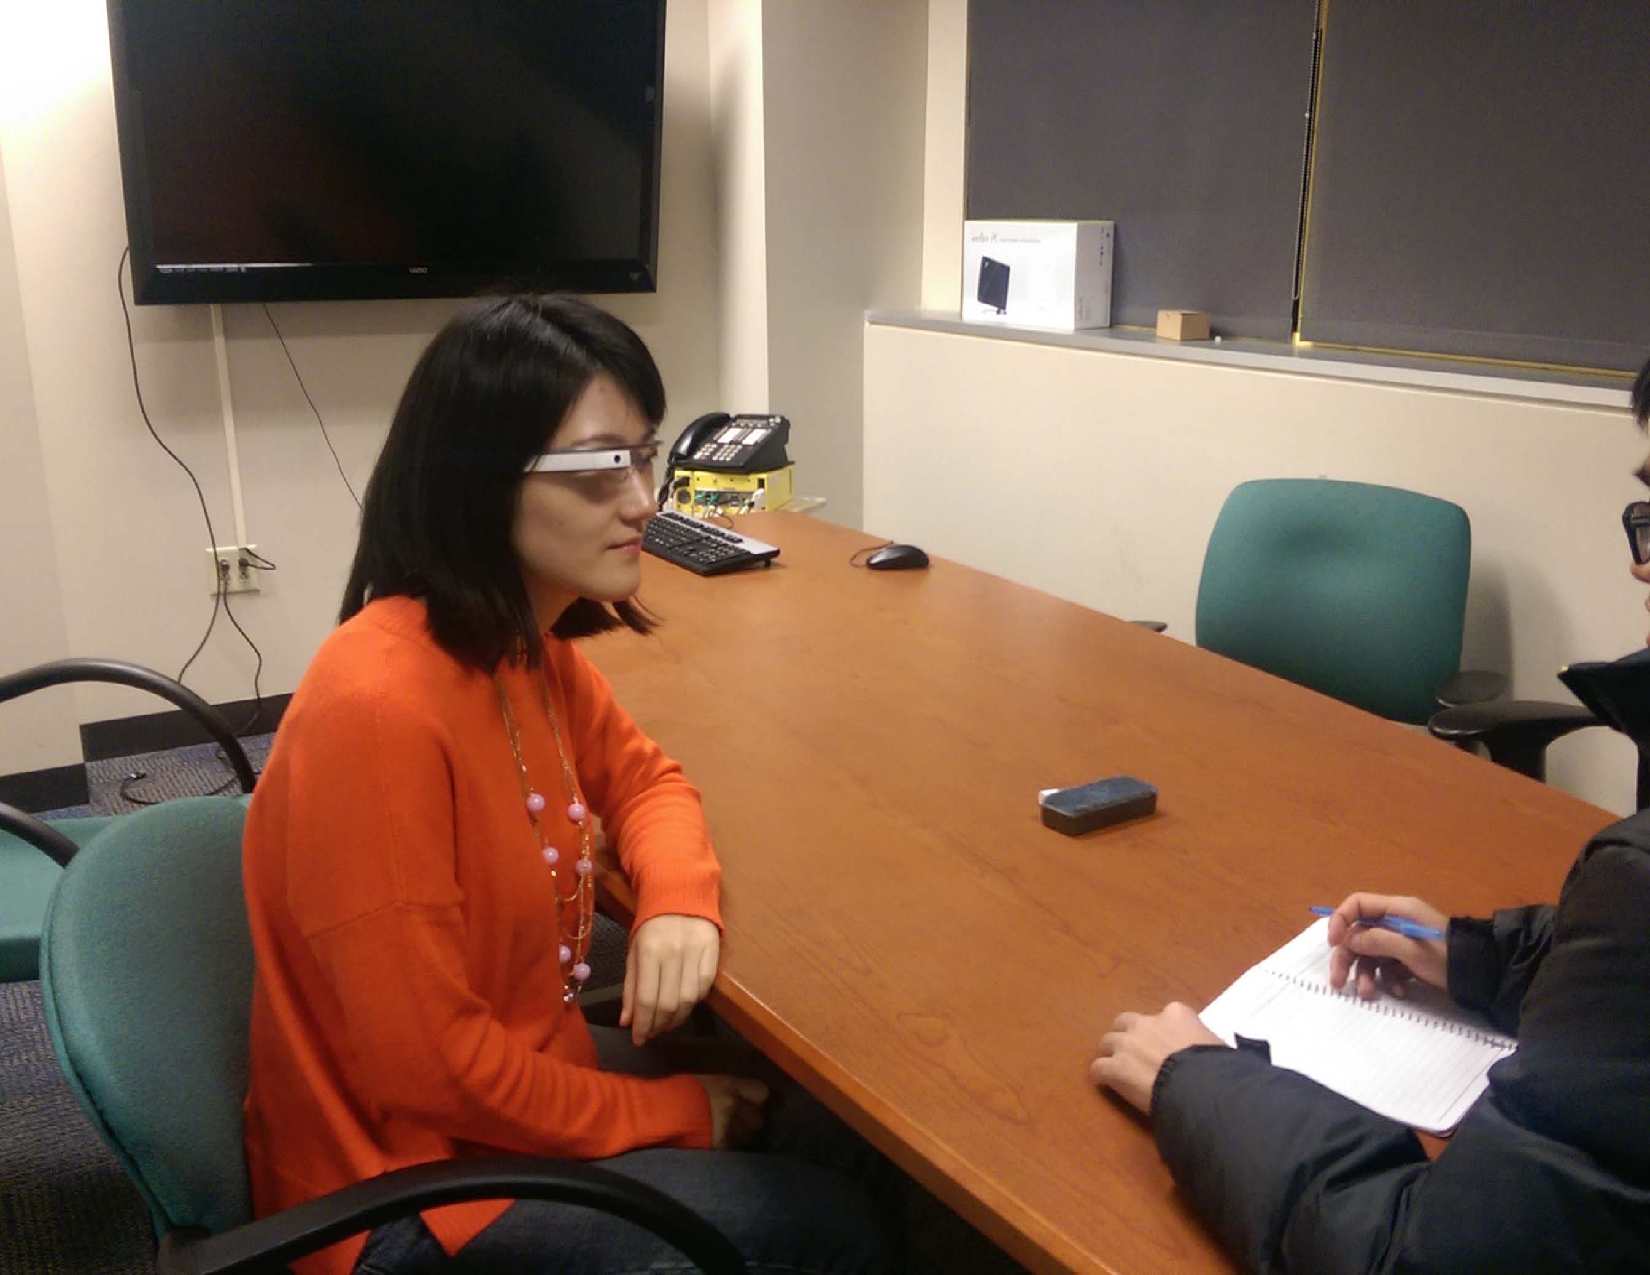
\includegraphics [width=.75\linewidth]{../mobisys_paper/fig/exp.pdf}
\caption{Our team member was collecting data with one of the participants. \label{fig:exp}}
\end{wrapfigure} 

The key to the success of this project is to collect data from a large and diverse set of participants, in different environments and contexts.  In this three-year project, we plan to collect data from *** subjects. We will make effort to recruit participants such that we have a balanced mix of gender, age, height, and handedness. We plan to pay each subject ***. 
 
In the data collection session, we will inform the participants of the potential risks involved in wearing Google Glass and collecting head-movement or eye blinking/winking/pulse data (e.g., feeling dizzy after head-movement for a period of time, not being able to see clearly if near-sighted, etc.), as well as the potential risks in wearing Moto 360 and collecting hand-movements/pulse data (e.g., wrist pain, ***). If they agree to participate, we will ask each subject to report their age and gender. We will help the subjects to wear the Google Glass and make head movements and eye blinking/winking while listening to the music track of their choice. We will also help the subjects to wear the Moto 360 and make wrist/hand movements while listening to the music track of their choice. Meanwhile, we will record the raw accelerometer data, raw gyroscope data, and the infra-red sensor data from the Google Glass.  Each recording session will be 10 seconds long, and we (the graduate students) will sit through each session with the subject to help him/her use the system properly, as shown in Figure~\ref{fig:exp}. After every 5 recording sessions, we will ask the subject to take a break to relax their muscle and regain energy. We will also split each subject's data collection session on different days, to include natural movement variability in the data sets. \emph{Both our system design and our data collection protocol have been approved by our Institutional Review Board.}


\subsection{Long Term App Evaluation}

\section{Work Plan}\label{subsec:plan}

